

\begin{slide}
\heading{A producer-consumer problem}

Consider the following producer-consumer problem (with a single producer and
single consumer).  The producer produces some data which it puts into a
``slot''.  The consumer gets the data and operates on it.  The consumer should
process each piece of data precisely once.  We want |put| and |get| operations
to support this. 

The consumer needs to be able to identify whether the data currently
in the slot is new or not, for which we use a boolean flag \SCALA{filled}.
%
\begin{itemize}
\item The producer waits until \SCALA{filled = false} before filling the slot,
and then sets \SCALA{filled} to \SCALA{true}.

\item The consumer waits until \SCALA{filled = true} before taking the data,
and then sets \SCALA{filled} to \SCALA{false}.
\end{itemize}

% (Alternatively, we could use an |Option| value, with |None| representing that
% the slot is empty.)
\end{slide}

%%%%%

\begin{slide}
\heading{Busy waiting}

Here's a definition that looks like it should work, but doesn't.

\begin{scala}
class Slot[T]{
  private var value = null.asInstanceOf[T] // current or previous item
  private var filled = false                 // if value valid?

  def put(v :T) = {
    while(filled){  } // spin
    value = v; filled = true
  }

  def get : T = {
    while(!filled){  } // spin
    val result = value; filled = false
    result
  }
}
\end{scala}
\end{slide}

%%%%%

\begin{slide}
\heading{Busy waiting}

The previous solution doesn't work because of compiler optimizations.  It
deadlocks after a few iterations.  I think  
\begin{scala}
    while(filled){  } 
\end{scala}
is ``optimized'' to something equivalent to
\begin{scala}
    if(filled){ while(true){} }
\end{scala}
by the JIT compiler.

Also, the compiler could reverse the order of the two assignments by |put|, or
could reverse the order of the two reads by |get|.  

Or the consumer could read a stale value of |value|, because of the use of
caches.
\end{slide}

%%%%%

\begin{slide}
\heading{Busy waiting}

Even if the code did work, it wouldn't be ideal.
%
% \begin{itemize}
% \item
The busy-waiting loop means both processes are using computational resources
unnecesarily.  This mechanism won't scale well, since if there are many
processes, they will be competing for access to the (limited) processors, and
also competing for use of the memory bus.

% \item
% Both processes need access to the object simultaneously, so we can't turn it
% into a monitor.  This doesn't matter in this case, but it would in others.

%% \item
%% The Java memory model makes no guarantee that the value of \SCALA{value} is
%% copied from the processor's cache to main memory.

%% \item
%% The compiler is allowed to perform optimisations to reverse the order of the
%% writes to \SCALA{value} and \SCALA{empty}.
%\end{itemize}

What we would like to do is arrange for the producer thread to wait (suspend)
until notified by the consumer thread that it can proceed.  Similarly, we
would like the consumer thread to wait (suspend) until notified by the
producer thread that it can proceed.
\end{slide}

%%%%%

\begin{slide}
\heading{Using {\scalashape wait} and {\scalashape notify}}

\begin{scala}
class Slot[T]{
  private var value = null.asInstanceOf[T] // current or previous item
  private var filled = false                 // if value valid?

  def put(v:T) = synchronized{
    while(filled) wait() // wait for the slot to be emptied
    value = v; filled = true
    notify()  // notify the consumer
  }

  def get : T = synchronized{
    while(!filled) wait() // wait for the slot to be filled
    val result = value; filled = false
    notify()  // notify the producer
    result
  }
}
\end{scala}
\end{slide}

%%%%%

\begin{slide}
\heading{{\scalashape wait} and {\scalashape notify}}

When a process executes \SCALA{wait()}, it is suspended and gives up
the lock.  If waits until another thread
in the same monitor executes \SCALA{notify()}, at which point it becomes
\emph{ready} to run.  

However, it cannot run until it obtains the lock on the monitor: the process
that performed the \SCALA{notify()} must release the lock; and the awakened
thread has to compete with other threads to obtain the lock.

Also, the implementation of |wait| is buggy.  Sometimes a thread doing a
|wait()| will wake up even though there was no |notify()|: a \emph{spurious
  wake-up}.
\end{slide}

%%%%%

\begin{slide}
\heading{Thread states}

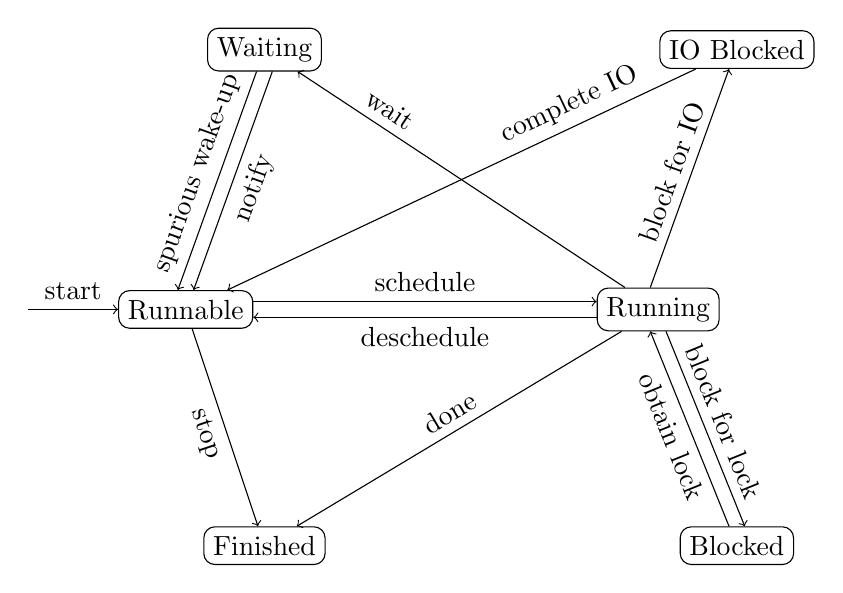
\begin{tikzpicture}
\draw(0,0) node[draw, rounded corners](runnable){Runnable};
\draw[<-] (runnable) -- node[above]{start} (-2,0);
%
\draw(6,0) node[draw, rounded corners](running){Running};
\draw[->] ([yshift = 1mm] runnable.east) -- node[above]{schedule} 
  ([yshift = 1mm] running.west);
\draw[->] ([yshift = -1mm] running.west) -- node[below]{deschedule} 
  ([yshift = -1mm] runnable.east);
% Waiting
\draw (1,3.3) node[draw, rounded corners](waiting){Waiting};
\draw[->] (running) -- node[above, sloped, near end]{\scalashape wait} (waiting);
\draw[->] ([xshift = -1mm] waiting.south) -- node[above, sloped]
  {spurious wake-up} ([xshift = -1mm] runnable.north);
\draw[->] ([xshift = 1mm] waiting.south) -- node[below, sloped]
  {\scalashape notify} ([xshift = 1mm] runnable.north);
%
\draw (1, -3) node[draw, rounded corners](finished){Finished};
\draw[->] (runnable) -- node[below, sloped]{stop} (finished);
\draw[->] (running) -- node[above, sloped]{done} (finished);
%
\draw(7, -3) node[draw, rounded corners](blocked){Blocked};
\draw[->] ([xshift = 1mm] running.south) -- 
  node[above, sloped]{block for lock} ([xshift = 1mm] blocked.north);
\draw[->] ([xshift = -1mm] blocked.north) -- node[below, sloped]{obtain lock} 
  ([xshift = -1mm] running.south);
% IO Blocked
\draw(7, 3.3) node[draw, rounded corners](IOblocked){IO Blocked};
\draw[->] ([xshift = -1mm] running.north) -- 
  node[above, sloped]{block for IO} ([xshift = -1mm] IOblocked.south);
\draw[->] ([xshift = 1mm] IOblocked) -- 
  node[above, sloped, near start]{complete IO} 
  (runnable);
\end{tikzpicture}

% \begin{center}
% \includegraphics[width=12cm]{Pics/threadStates.eps}
% \end{center}
\end{slide}

%%%%%

\begin{slide}
\heading{{\scalashape wait} and {\scalashape notify}}

Normally, a process performs a \SCALA{wait} because some condition~\SCALA{cond}
is false, and it needs to wait for~\SCALA{cond} to become true.  

Normal practice is for another thread to perform a |notify| only when the
condition becomes true.

However, because of the possibility of spurious wake-ups, the awoken thread
should re-check the  condition~\SCALA{cond}.  The correct form of waiting is
%
\begin{scala}
  while(!cond) wait()
\end{scala}

Further, even without the possibility of spurious wake-ups, some third thread
might have run before the awoken thread, and so made the condition false. 

% Further, sometimes a thread will wake up without being notified, due to bugs
% in the implementation of Java --- a so-called \emph{spurious wakeup}.  These
% occur rarely in practice, but you should still guard against them, for example
% by using the above form of waiting.
\end{slide}

%%%%%

\begin{slide}
\heading{Multiple producers and consumers}

Suppose we run the |Slot| with multiple producers and consumers.  It turns out
that previous implementation works incorrectly.
%
Consider the following execution, if |notify| is used.
%
\begin{enumerate}
\item Two consumers run, and both have to wait.

\item Producer~1 runs, sets |filled = true|, wakes up consumer~1, and returns.

\item Producer~2 runs, but has to wait.

\item Consumer~1 runs, sets |filled = false|, calls |notify()| which wakes up
consumer~2, and returns.

\item Consumer~2 runs, finds |filled = false|, so waits again. 
\end{enumerate}
%
Now producer~2 and consumer~2 are both waiting, but they should have been able
to exchange data. 

% If consumer~1 calls |notifyAll|, things will work correctly. 
\end{slide}

%%%%%

\begin{slide}
\heading{\scalashape notifyAll}


\SCALA{notify()} wakes up just one thread (if there is one waiting).  By
contrast, \SCALA{notifyAll()} wakes up \emph{all} threads waiting in this
monitor. 

Note that \SCALA{notifyAll()} is an expensive operation: all the waiting
threads will be awoken, obtain the lock, check the guard on their wait loop,
and normally all but one will immediately do another \SCALA{wait}.
\end{slide}

%%%%%

\begin{slide}
\heading{A slot for multiple producers and consumers}

\begin{scala}
class Slot2[T]{
  private var value = null.asInstanceOf[T]
  private var filled = false

  def put(v:T) = synchronized{
    while(filled) wait()
    value = v; filled = true; notifyAll()
  }

  def get : T = synchronized{
    while(!filled) wait()
    filled = false; notifyAll(); value
  }
}
\end{scala}
%
\end{slide}

%%%%%

\begin{slide}
\heading{A slot for multiple producers and consumers}

Note that in this case it would be necessary for an awoken thread to recheck
the condition even if spurious wake-ups didn't exist: it is possible that some
other thread has run and invalidated the condition in the meantime.

Having to use |notifyAll| is inefficient.  It would be better if |get| could
target a |notify| towards a |put|, and vice versa.  We'll see a way to achieve
this effect in a later chapter.
\end{slide}

%%%%%

\begin{slide}
\heading{Signal-and-continue versus signal-and-wait}

Note that Scala (like Java) uses \emph{signal-and-continue} semantics: when a
process signals, it continues to hold the lock on the monitor; the
awakened process must wait to get the lock.  That means that we could have
written |get| as 
%
\begin{scala}
  def get : T = synchronized{
    while(!filled) wait() // wait for the slot to be filled
    filled = false
    notify() // notify the producer
    value
  }
\end{scala}

By contrasts, some systems use \emph{signal-and-wait} semantics, where the
process that signals also gives up the lock; the awakened process runs.
\end{slide}

%%%%%

% \begin{slide}
% \heading{Exercise}

% Adapt the |Slot| example to hold an (unbounded) partial queue of data.
% \end{slide}


%%%%%

% \begin{slide}
% \heading{Caches and memory optimisations}

% The original version of the slot has some additional subtle problems:
% %
% \begin{itemize}
% \item
% The Java memory model makes no guarantee that the value of \SCALA{value} is
% copied from the processor's cache to main memory.

% \item
% The compiler is allowed to perform optimisations to reverse the order of the
% writes to \SCALA{value} and \SCALA{empty}.
% \end{itemize}
% \end{slide}

%%%%%

\begin{slide}
\heading{Java Memory Model}

Recall that the original version of the slot has some  subtle problems caused
by the Java Memory Model.  The use of |wait| and |notify| avoids
these. 

When a thread exits a |synchronized| block (either at the end of a
procedure, or be performing a \SCALA{wait}), it \emph{publishes} the
values in the cache, making them available to other threads.

When a thread enters a |synchronized| block (either initially, or after
receiving a \SCALA{notify}), it \emph{subscribes} to all variables
published by other threads on the same monitor.

Compiler optimisations must respect this
semantics.
%% \footnote{\url{http://www.cs.umd.edu/~pugh/java/memoryModel/jsr-133-faq.html}}

\vfill
\end{slide}


%%%%%

\begin{slide}
\heading{{\scalashape wait} and {\scalashape notify}}

\SCALA{wait(t)} acts like \SCALA{wait()}, except it will wake up after
\SCALA{t}ms, if it hasn't been woken by a \SCALA{notify} in the meantime.
This can be used to implement timeouts.  

%% \SCALA{notify()} wakes up just one thread (if there is one waiting).  By
%% contrast, \SCALA{notifyAll()} wakes up \emph{all} threads waiting in this
%% monitor. 

%% See the API documentation for \SCALA{Scala.AnyRef} and
%% \SCALA{java.lang.Object} for more details.

%% Note that \SCALA{notifyAll()} is an expensive operation: all the waiting
%% threads will be awoken, obtain the lock, check the guard on their wait loop,
%% and normally all but one will immediately do another \SCALA{wait}.

All calls to each of |wait|, |notify| and |notifyAll| must be from inside a
|synchronized| block.
\end{slide}
